\documentclass[11pt]{amsart}
\usepackage{color}
\usepackage{color}
\usepackage{tikz}
\usetikzlibrary{decorations.markings, hobby, knots}
\usepackage{pgffor}

\begin{document}

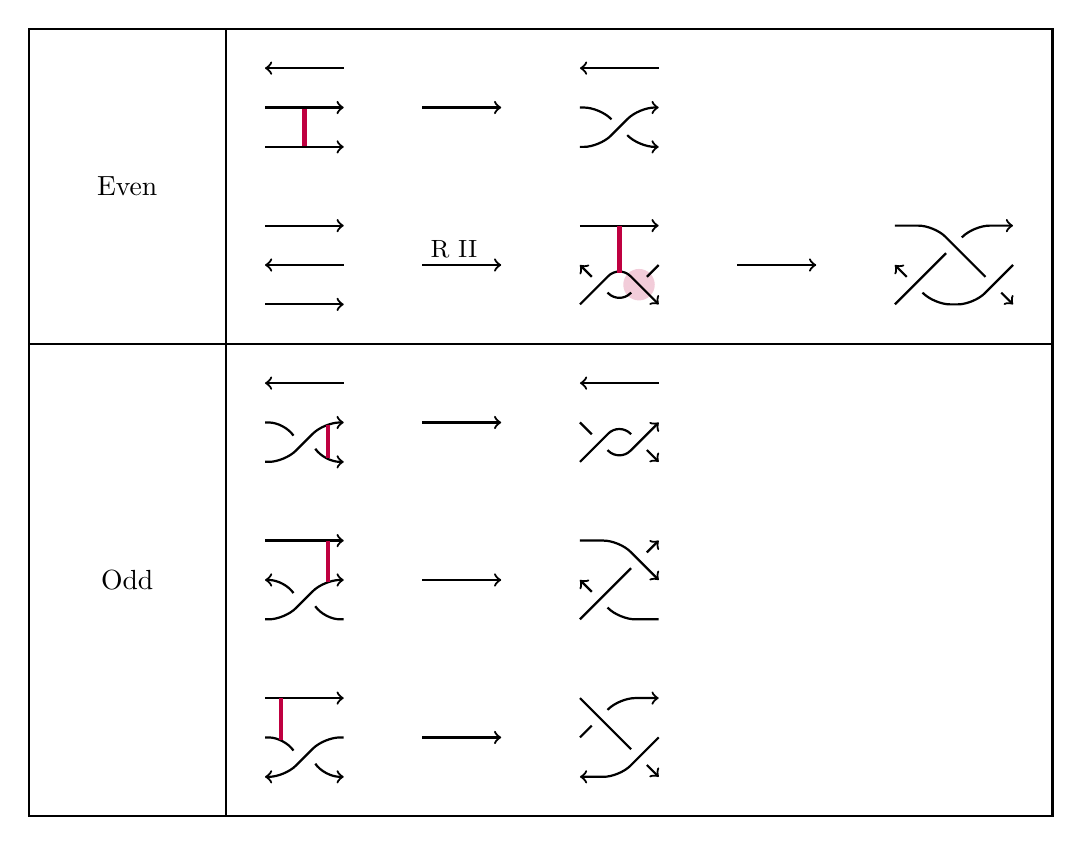
\begin{tikzpicture}[thick]
%Case 1
%Before link fix move

\draw[purple, ultra thick] (.5,0) -- (.5,.5);
\draw[->] (0,0) -- (1,0);
\draw[->] (0,.5) -- (1,.5);
\draw[->] (1,1) -- (0,1);

\draw [->] (2,.5) -- (3,.5);

%After Twist
\begin{scope}[xshift = 4cm]

\draw[rounded corners=2mm, ->] (0,0) -- (.25,0) -- (.75,.5) -- (1,.5);
\draw[rounded corners = 2mm] (0,.5) -- (.25,.5) -- (.4,.35);
\draw[rounded corners = 2mm, ->] (.6,.15) -- (.75,0) -- (1,0);
\draw[->] (1,1) -- (0,1);
\end{scope}

\begin{scope}[yshift = -2cm]
\draw[->] (0,0) -- (1,0);
\draw[<-] (0,.5) -- (1,.5);
\draw[->] (0,1) -- (1,1);

\draw [->] (2,.5) -- (3,.5);
\draw (2.4,.7) node{\small{R II}};

\begin{scope}[xshift = 4cm]
\fill[white!80!purple] (0.75,0.25) circle (.2cm);
\draw[->, rounded corners = 2mm] (0,0) -- (.5,.5) -- (1,0);
\draw (1,.5) -- (.85,.35);
\draw[rounded corners = 2mm] (.65,.15) -- (.5,0) -- (.35,.15);
\draw[->] (.15,.35) -- (0,.5);
\draw[->] (0,1) -- (1,1);
\draw[purple, ultra thick] (0.5,.4) -- (0.5,1);

\draw [->] (2,.5) -- (3,.5);

\end{scope}

\begin{scope}[xshift = 8cm, rounded corners = 2mm]

\draw (0,0) -- (.65,.65);
\draw[->] (.85,.85) -- (1,1) -- (1.5,1);
\draw[<-] (0,.5) -- (.15,.35);
\draw (.35,.15) -- (.5,0) -- (1,0) -- (1.5,.5);
\draw (0,1) -- (.5,1) -- (1.15,.35);
\draw[->] (1.35,.15) -- (1.5,0);
    
\end{scope}

\end{scope}
%Row 3
\begin{scope}[yshift=-4cm]

\draw[rounded corners = 2mm, ->] (0,0) -- (.25,0) -- (.75,.5) -- (1,.5);
\draw[rounded corners = 2mm] (0,.5) -- (.25,.5) -- (.35,.35);
\draw[rounded corners = 2mm, ->] (.65,.15) -- (.75,0) -- (1,0);
\draw[->] (1,1) -- (0,1);
\draw[purple, ultra thick] (.8,.47) -- (.8,.05);

\draw [->] (2,.5) -- (3,.5);

\begin{scope}[xshift = 4cm, rounded corners = 2mm]
    \draw (0,0) -- (.5,.5) -- (.65,.35);
    \draw[->] (.85,.15) -- (1,0);
    \draw (0,.5) -- (.15,.35);
    \draw[->] (.35,.15) -- (.5,0) -- (1,.5);
    \draw[->] (1,1) -- (0,1);
\end{scope}

\end{scope}

%Row 4
\begin{scope}[yshift=-6cm]

\draw[rounded corners = 2mm, ->] (0,0) -- (.25,0) -- (.75,.5) -- (1,.5);
\draw[rounded corners = 2mm, <-] (0,.5) -- (.25,.5) -- (.35,.35);
\draw[rounded corners = 2mm] (.65,.15) -- (.75,0) -- (1,0);
\draw[<-] (1,1) -- (0,1);
\draw[purple, ultra thick] (.8,.47) -- (.8,1);

\draw [->] (2,.5) -- (3,.5);

\begin{scope}[xshift = 4cm, rounded corners = 2mm]
    \draw (0,0) -- (.65,.65); 
    \draw[->] (.85,.85) -- (1,1);
    \draw[<-] (0,.5) -- (.15,.35);
    \draw (.35,.15) -- (.5,0) -- (1,0);
    \draw[->] (0,1) -- (.5,1) -- (1,.5);
\end{scope}

\end{scope}

%Row 5
\begin{scope}[yshift=-8cm]

\draw[rounded corners = 2mm, <-] (0,0) -- (.25,0) -- (.75,.5) -- (1,.5);
\draw[rounded corners = 2mm] (0,.5) -- (.25,.5) -- (.35,.35);
\draw[rounded corners = 2mm,->] (.65,.15) -- (.75,0) -- (1,0);
\draw[<-] (1,1) -- (0,1);
\draw[purple, ultra thick] (.2,.47) -- (.2,1);

\draw [->] (2,.5) -- (3,.5);

\begin{scope}[xshift = 4cm, rounded corners = 2mm]
    \draw (0,1) -- (.65,.35); 
    \draw[->] (.85,.15) -- (1,0);
    \draw (0,.5) -- (.15,.65);
    \draw[->] (.35,.85) -- (.5,1) -- (1,1);
    \draw[<-] (0,0) -- (.5,0) -- (1,.5);
\end{scope}

\end{scope}

\draw (-3,1.5) rectangle (10,-8.5);
\draw (-3,-2.5) -- (10,-2.5);
\draw (-.5,1.5) -- (-.5,-8.5);
\draw (-1.75 ,-.5) node {Even};
\draw (-1.75, -5.5) node {Odd};

\end{tikzpicture}

\end{document}